\section{Introduction}

\begin{frame}{Writing Secure Java Code}
	Java is one of the most widely used programming languages, and many security-critical applications are written in Java.
	
	Applications interacting with sensitive information must ensure the \textit{confidentiality} of that information. They can do this by:
	
	\begin{itemize}
		\item Following the Oracle Secure Coding Guidelines
		\item Running their application with a \texttt{SecurityManager} installed
		\item Following the Principle of Least Privilege
	\end{itemize}
	
	Java's Security Model provides APIs to secure applications with \textbf{access control}, but has no direct mechanisms for control of \textbf{information flows}.
\end{frame}

\begin{frame}{Why Does Information Flow Matter?}

	\begin{figure}
		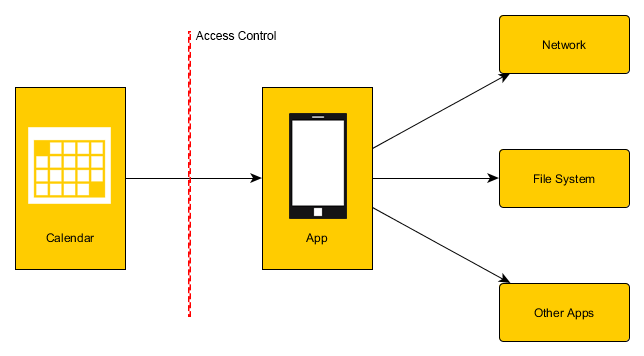
\includegraphics[scale=0.5]{content/images/calendar_flow.png}
		\caption{Example -- A Meeting Scheduler Application}
	\end{figure}
	
	\note{
	Consider an app that lets you schedule meetings. You grant it the `Calendar' and `Network' permissions on your phone. But once it has that permission, the app can do \textit{anything it likes} with your calendar, including sending your entire schedule over the network.
	
	With access control, you grant access and your security ends there. What we really want to do is control where that information \textit{flows}. In this case, we want your app to be able to use your calendar to check that your schedule is free, but we don't want it to be able to save or send that information elsewhere.
	
	As it happens, there exist \textbf{Information Flow} security models, which aim to provide \textit{provable} confidentiality in this fashion.	
	}
\end{frame}

\begin{frame}{Information Flow and Access Control}
	Many systems implement \textbf{access control} mechanisms, which place restrictions based on the \textit{permissions} of a user or of calling code, but which cannot restrict how that information \textit{propagates} once released \cite{ifbackground:sabelfeld}.
	
	\textbf{Information flow} mechanisms instead control access by enforcing that some \textit{policy} on the data is upheld.
	
	In short, access control puts controls on the \textit{calling code}, where information flow puts controls on the \textit{data}.
\end{frame}

%\begin{frame}{Java is Vulnerable}
%	\begin{columns}
%		\column{0.55\textwidth}
%			37 vulnerabilities in the JRE were recorded in the US National Vulnerability Database in 2016.\newline
%			
%			13 were listed as `critical', with a CVSS score $ > $ 9.0, indicating complete compromise of Confidentiality and Integrity \cite{nvd:jdk2016cvss9}.\newline
%			
%			This is in the \textit{JRE alone}, without considering the thousands of Java libraries and applications in existence.
%		\column{0.45\textwidth}
%		\begin{figure}
%			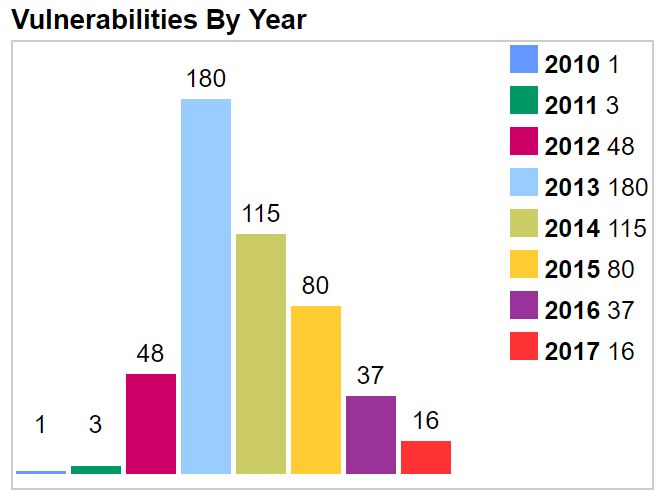
\includegraphics[scale=0.25]{content/images/cvedetails_vulnsperyear.png}
%			\caption{Total CVEs by year \cite{cvedetails:jdk2016}}
%		\end{figure}
%	\end{columns}	
%\end{frame}



\begin{frame}{Thesis Topic}
	\begin{block}{Key Thesis Question}
		Can Information Flow be used to provide practical improvements to the confidentiality of Java programs?
	\end{block}
	
	This thesis aims to evaluate the theory of information flow-based security and current implementations of it to determine:
	
	\begin{enumerate}
		\item What security benefits do current Information Flow implementations provide?
		\item What burden do they place on the programmer?
		\item What would future implementations need to be practical for real world applications? 
	\end{enumerate}
\end{frame}